\documentclass[letterpaper]{article} % DO NOT CHANGE THIS
\usepackage{aaai2027}  % DO NOT CHANGE THIS (camera-ready style, as the Student Abstract call requires)
% The serif, sans-serif, and monospaced fonts are loaded automatically by
% aaai2027.sty (newtxtext, helvet, courier). DO NOT add any font package.
\usepackage[hyphens]{url}  % DO NOT CHANGE THIS
\usepackage{graphicx} % DO NOT CHANGE THIS
\urlstyle{rm} % DO NOT CHANGE THIS
\def\UrlFont{\rm}  % DO NOT CHANGE THIS
\usepackage{natbib}  % DO NOT CHANGE THIS AND DO NOT ADD ANY OPTIONS TO IT
\usepackage{caption} % DO NOT CHANGE THIS AND DO NOT ADD ANY OPTIONS TO IT
\frenchspacing  % DO NOT CHANGE THIS
\usepackage{booktabs}
\usepackage{amsmath}
\usepackage{amssymb}
%
% Keep the \pdfinfo as shown here. There's no need
% for you to add the /Title and /Author tags.
\pdfinfo{
/TemplateVersion (2027.1)
}

% Section numbers must stay off in extended abstracts.
\setcounter{secnumdepth}{0}

% AAAI-27 Student Abstract and Poster Program: 2 pages INCLUDING references,
% camera-ready style, primary author contact details on the first page.
% Single-file source by design (the camera-ready archive allows no \input).

\title{FactorJEPA on DENSEWORLD-115k: Can a World Model Predict Crowded, Chaotic South Asian Streets?}

\author{
    Gaytri Jena\textsuperscript{\rm 1}\thanks{All authors conducted this work independently, outside their roles and employment at their respective companies.},
    Kapil Wanaskar\textsuperscript{\rm 2},
    Aman Chadha\textsuperscript{\rm 3},
    Vini{}ja Jain\textsuperscript{\rm 4},  % {} breaks the "ij" ligature
    Vasu Sharma\textsuperscript{\rm 5},
    Amitava Das\textsuperscript{\rm 6}
}
\affiliations{
    % Student Abstract call: the PRIMARY author (first) needs affiliation, postal
    % address, phone, URL and e-mail on the page; co-authors need name + affiliation.
    % Institutional contact, as the call's "postal address, phone number" for the primary
    % author: the School of Information's public mailing address and main line
    % (ischool.berkeley.edu/about/contactus, checked 2026-09-24), not a home address.
    \textsuperscript{\rm 1}UC Berkeley School of Information (MIDS), 102 South Hall \#4600, Berkeley, CA 94720-4600, USA, +1 (510) 642-1464\quad
    \textsuperscript{\rm 2}San Jose State University, USA\quad
    \textsuperscript{\rm 3}Apple, USA\quad
    \textsuperscript{\rm 4}Meta, USA\quad
    \textsuperscript{\rm 5}PocketFM, USA\quad
    \textsuperscript{\rm 6}Pragya Lab, BITS Pilani Goa, India\\
    gaytri\_jena@ucberkeley.edu, \url{https://kapilw25.github.io/factorjepa}
}

\begin{document}

\maketitle

\begin{abstract}
Joint Embedding Predictive Architectures (JEPA) forecast the future in embedding space, yet they are mostly evaluated on lower-density, lane-structured traffic. We study DENSEWORLD, the regime of crowded South Asian streets with soft spatial boundaries, heterogeneous agents, persistent occlusion, and negotiated motion, through DENSEWORLD-115k: 115,687 clips (about 1,000 hours) from 22 Indian cities. FactorJEPA replaces the monolithic V-JEPA predictor with separate layout, agent, and interaction channels. After full 115k-clip training it separates from the strongest competing adaptation method on all four diagnostics of predictive structure by 13.9 to 43.3 widths of the paired 95\% confidence interval, with rankings that replicate across 2B and 1B backbones (Spearman $\rho \geq 0.895$), while competitors stay ahead on temporal coherence.
\end{abstract}

\begin{links}
    \link{Paper}{https://arxiv.org/abs/2608.01049}
    \link{Code}{https://github.com/kapilw25/factorjepa}
    \link{Dataset}{https://huggingface.co/datasets/anonymousML123/denseworld-115k}
\end{links}

\section{Problem}

Video world models such as V-JEPA 2.1 \cite{murlabadia2026vjepa21} predict masked or future content as embeddings instead of pixels. Their predictors are monolithic, so nothing forces layout, agents, and interactions to stay distinguishable inside the predicted future, which matters most where these factors are tightly coupled. DENSEWORLD is such a regime: road edges are negotiated rather than marked, pedestrians, two-wheelers, auto-rickshaws, carts, and animals share one right of way, clutter keeps agents partially hidden, and motion follows social negotiation more than lane rules. DENSEWORLD holds 115,687 privacy-filtered clips of 6 to 13 seconds from drive-through, walk-through, and aerial footage (Figure~\ref{fig:teaser}, top), and shows consistently higher agent density and occupancy than BDD100K and nuScenes on matched scene types.

\section{Key Results}

\paragraph{Protocol.}
We adapt V-JEPA 2.1 at 2B and 1B parameters on a matched stratified 10k-clip set, and the 1B model also on the full 115k-clip corpus. FactorJEPA is compared with the frozen backbone, full fine-tuning, linear probing then fine-tuning (LP-FT), continual self-supervised learning, LoRA \cite{hu2022lora}, DoRA \cite{liu2024dora}, and Auto-RGN \cite{lee2023surgical} under identical clips, masking, steps, and splits. Headline evaluation uses a city-disjoint audit split with independently annotated agents, visibility, interactions, and intervention regions, so no evaluator reuses the training targets.

% Declared here, in page 1's RIGHT column, on purpose: a figure* declared in the
% left column of the title page trips the style file's footnote/copyright budget
% (27 pt overfull vbox into the bottom margin); declared here it lands cleanly at
% the top of page 2. Measured 2026-09-21.
\begin{figure*}[t]
\centering
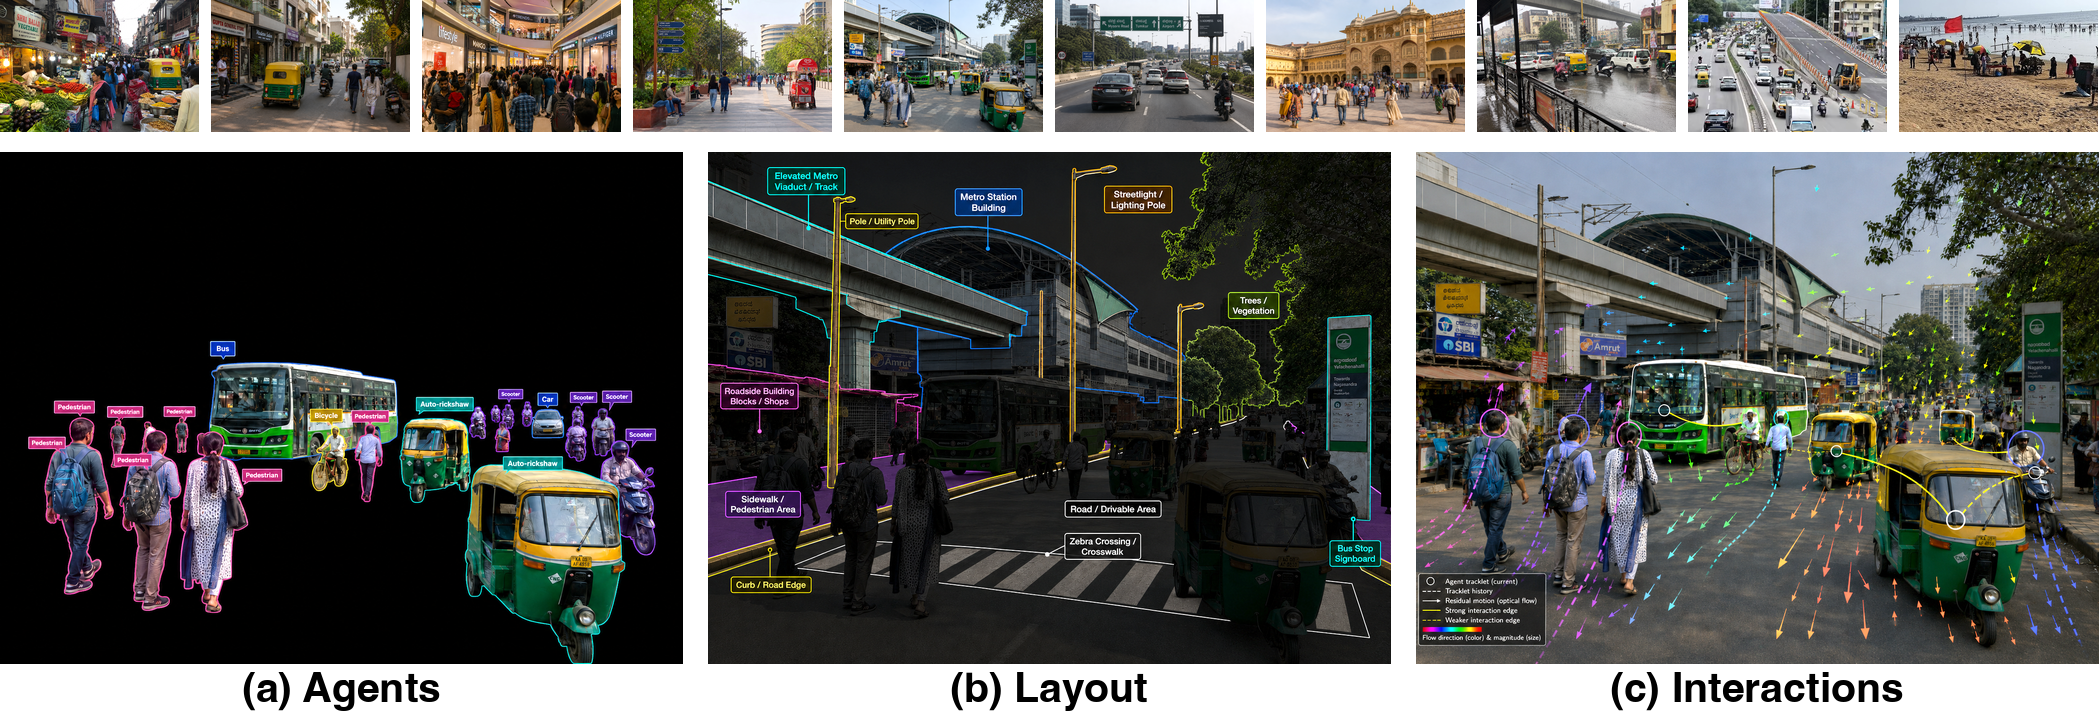
\includegraphics[width=\textwidth]{figures/denseworld_teaser.png}
\caption{DENSEWORLD at a glance. Top: ten scene types, left to right: market, residential, commercial, promenade, transit, highway, heritage, junction, flyover, and beach, from 115,687 clips across 22 Indian cities. Bottom: one scene factorized into (a) agents, (b) layout with agents suppressed, and (c) interactions: circles mark tracked agents, arrows encode motion (colour: direction; length: magnitude), and solid or dashed edges mark stronger or weaker coupling.}
\label{fig:teaser}
\end{figure*}

\paragraph{Diagnostics.}
Future-frame L1: error between predicted and target future embeddings. Causal L1: whether a controlled edit to an annotated region changes the predicted future as it changes the target. Mask-ratio slope: error growth as evidence is removed. Motion cosine: linear decodability of motion. Margins are in widths of the paired 95\% BCa bootstrap confidence interval; 1 or more is separated.

% Every number below is produced by src/m13_eval_plot.py's best-arm logic
% (_xb_best over _XB_METRICS) on the three tracked eval_metrics.json snapshots
% (iter18 v3 2B 10k, iter18 v5_1B 1B 10k, iter19 1B 115k), the same cells the
% forest plot showed. Bold = the better score of each pair by the metric's
% direction; a pair equal at three decimals bolds neither (five such pairs,
% all with margins inside one CI width). The rival superscript is the arm
% _xb_best picked: L peft_lora, D peft_dora, F full_ft, C pretrain (continual
% SSL), Z frozen. Ours varies per cell (mostly surgical_3stage_DI_diheavy;
% surgery_raw, intervene and WiSE-FT merges win some 10k cells) and is not
% annotated: the abstract never introduces those variants. Margins in
% paired-CI widths live in the abstract and the Findings text. Single column
% at 9 pt with a 2-pt column gap (\setlength{\tabcolsep} is the one \setlength
% the kit permits); the [!t] float lands under Figure 1 on page 2.
\begin{table}[!t]
\centering
\small
\setlength{\tabcolsep}{2pt}
\begin{tabular}{lrrrrrr}
\toprule
 & \multicolumn{2}{c}{2B$\cdot$10k} & \multicolumn{2}{c}{1B$\cdot$10k} & \multicolumn{2}{c}{1B$\cdot$115k} \\
\cmidrule(lr){2-3}\cmidrule(lr){4-5}\cmidrule(lr){6-7}
Diagnostic & Ours & Rival & Ours & Rival & Ours & Rival \\
\midrule
future-frame L1 ($\downarrow$) & \textbf{0.496} & 0.504\textsuperscript{L} & \textbf{0.587} & 0.596\textsuperscript{L} & \textbf{0.573} & 0.589\textsuperscript{L} \\
causal-block L1 ($\downarrow$) & \textbf{0.528} & 0.533\textsuperscript{L} & \textbf{0.611} & 0.617\textsuperscript{L} & \textbf{0.597} & 0.607\textsuperscript{L} \\
mask-ratio slope ($\downarrow$) & \textbf{0.053} & 0.054\textsuperscript{L} & \textbf{0.052} & 0.053\textsuperscript{D} & \textbf{0.047} & 0.058\textsuperscript{L} \\
motion-cos ($\uparrow$) & 0.135 & \textbf{0.244}\textsuperscript{F} & 0.060 & \textbf{0.090}\textsuperscript{F} & \textbf{0.097} & 0.078\textsuperscript{L} \\
\midrule
temporal-order ($\uparrow$) & \textbf{0.953} & 0.947\textsuperscript{Z} & 0.925 & \textbf{0.927}\textsuperscript{C} & \textbf{0.918} & 0.915\textsuperscript{Z} \\
pace ($\uparrow$) & \textbf{0.736} & 0.724\textsuperscript{L} & \textbf{0.731} & 0.729\textsuperscript{Z} & 0.703 & 0.703\textsuperscript{L} \\
action top-1 ($\uparrow$) & 0.508 & \textbf{0.528}\textsuperscript{C} & 0.483 & \textbf{0.509}\textsuperscript{F} & 0.567 & \textbf{0.572}\textsuperscript{L} \\
arrow-of-time ($\uparrow$) & 0.964 & \textbf{0.965}\textsuperscript{Z} & 0.964 & \textbf{0.965}\textsuperscript{Z} & 0.955 & \textbf{0.975}\textsuperscript{Z} \\
TCC $\tau$ ($\uparrow$) & 0.288 & \textbf{0.292}\textsuperscript{Z} & 0.323 & \textbf{0.334}\textsuperscript{Z} & 0.380 & \textbf{0.400}\textsuperscript{Z} \\
exposure-bias ($\downarrow$) & 0.038 & 0.038\textsuperscript{C} & \textbf{0.034} & 0.036\textsuperscript{D} & 0.038 & \textbf{0.035}\textsuperscript{L} \\
rollout drift ($\downarrow$) & 0.008 & 0.008\textsuperscript{C} & 0.005 & 0.005\textsuperscript{D} & 0.007 & \textbf{0.006}\textsuperscript{L} \\
L1-vs-$\Delta t$ ($\downarrow$) & 0.006 & 0.006\textsuperscript{C} & 0.008 & \textbf{0.007}\textsuperscript{Z} & 0.009 & \textbf{0.007}\textsuperscript{Z} \\
TCC cycle ($\downarrow$) & \textbf{2.092} & 2.111\textsuperscript{Z} & 2.240 & \textbf{2.195}\textsuperscript{Z} & 2.806 & \textbf{2.132}\textsuperscript{Z} \\
\bottomrule
\end{tabular}
% Legend as a table note (9 pt, the kit's table minimum), between the body and
% the caption, so the caption stays a description.
\par\smallskip
{\small\raggedright
Rival superscript: L LoRA, D DoRA, F full fine-tuning, C continual self-supervised learning, Z frozen backbone. At 115k only LoRA and the frozen backbone were trained as rivals.\par}
\caption{Scores of the best FactorJEPA arm (Ours) and of its strongest rival on all 13 diagnostics, for V-JEPA~2.1 at 2B and 1B on the stratified 10k set and at 1B on the full 115k set. Above the rule: the four diagnostics of predictive structure; below: the rest, where the rival often leads. Bold: the better score of each pair (neither when equal at this precision); arrows give the better direction.}
\label{tab:headline}
\end{table}

\paragraph{Findings.}
With limited data (Table~\ref{tab:headline}), FactorJEPA separates on Future-frame L1 and Causal L1 at both scales and on Mask-ratio slope at 1B, while Motion cosine favors generic fine-tuning. Full 115k-clip training reverses that deficit: FactorJEPA then separates on all four diagnostics, so the prediction versus motion trade-off depends on data, not on the factorization. Rankings replicate from the 2B to the roughly half-cost 1B backbone (Spearman $\rho \geq 0.895$). The gain is targeted, not universal: below the rule in Table~\ref{tab:headline}, the best rival stays ahead at 115k on six diagnostics (rollout drift, exposure bias, L1-versus-$\Delta t$ decay, arrow-of-time, and the two TCC measures) by 8.3 to 146.5 interval widths, so temporal coherence remains the open weakness.

\section{Method}

FactorJEPA keeps the pretrained V-JEPA 2.1 encoder, its momentum target encoder, the masking policy, and the prediction targets, and replaces only the predictor. For each target token it predicts layout, agent, and interaction coordinates $C_L$, $C_A$, $C_I$ (Figure~\ref{fig:teaser}, bottom) and composes the future embedding through learned dictionaries, $\widehat Y = C_L A_L^{\top} + C_A A_A^{\top} + C_I A_I^{\top}$. A soft visibility gate down-weights occluded agents instead of discarding them, and interaction coordinates are sparse weighted sums over candidate agent pairs. Factor heads are anchored to layout, agent, visibility, and interaction targets from a frozen DINOv2 pipeline \cite{oquab2024dinov2}, on the training split only, and a penalty on cross-channel covariance and kernel alignment limits shortcut mixing. The objective adds separation, sparsity, visibility, and factor-supervision terms to the JEPA loss, and only the predictor and the top $K$ encoder blocks are trained. The work bridges video self-supervised learning, multi-agent scene understanding, and urban mobility in a setting current world-model benchmarks rarely cover.

% The kit allows references, and only references, at \small (9 pt) when the page limit is exceeded.
{\small
\bibliography{factorjepa}
}

\end{document}
